\begin{figure}[!htbp]
\centering
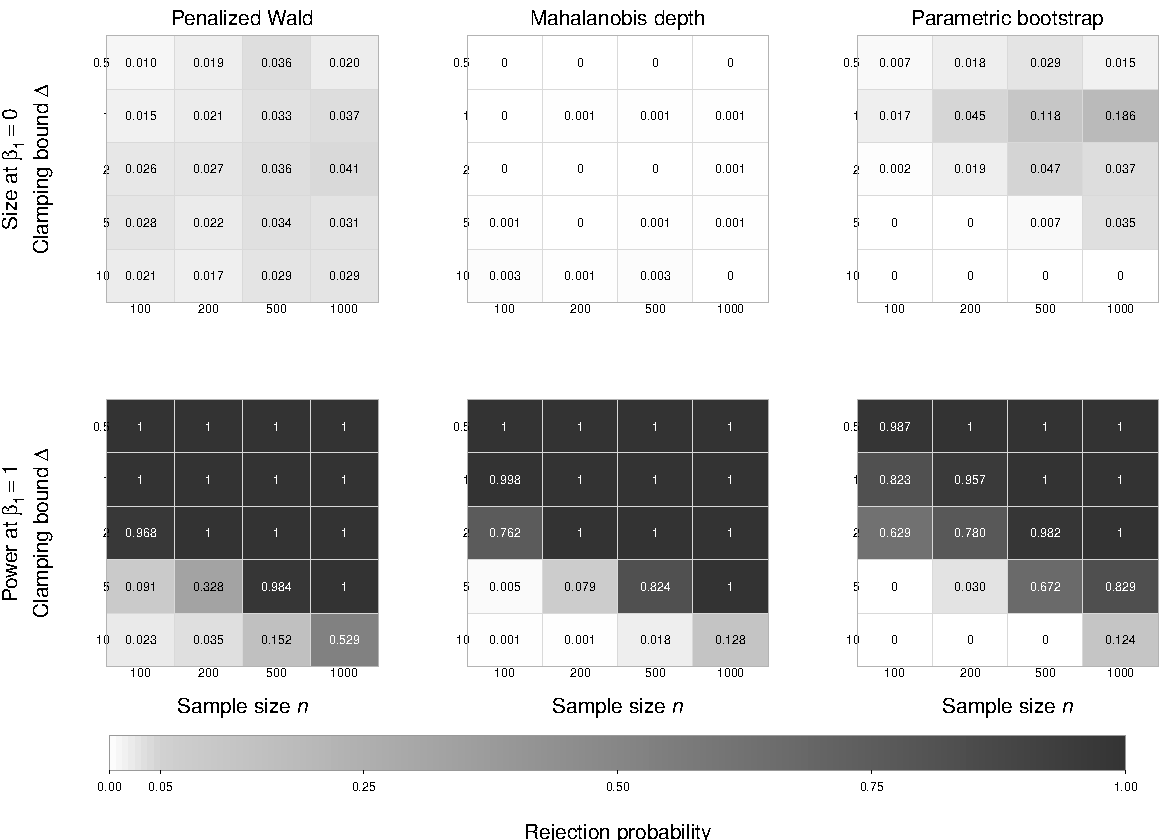
\includegraphics[width=0.95\linewidth]{results/figures/fig_delta_sensitivity.pdf}
\caption{Sensitivity to the clamping range. The first row of panels shows
empirical size at $\beta_1^\ast=0$ and the second shows power at
$\beta_1^\ast=1$. Rows within each heat map are clamping bounds and columns
are sample sizes, with $1000$ replications per cell. Unresolved Penalized
Wald tests are counted as non-rejections. The grey scale breaks at $0.05$:
dark cells in the size panels have observed rejection rates above nominal,
which alone does not establish population size inflation. The bound
$0.04975$ applies to the exact finite-$R$ rank tests, not to the bootstrap.
Larger clamping bounds retain more of the latent observations but increase
the second-moment noise scale as $\Delta^2/n$. On this grid, Penalized Wald
power is high at the smaller bounds and decreases at larger bounds.
Comparator values are those reported by \citet[Fig.~6]{awan2024simulation},
restricted to this design. Alternative rejection probabilities are not
size-matched power comparisons when the procedures' null rejection rates
differ.}
\label{fig:delta-sensitivity}
\end{figure}
